Un SoC est composé de blocs correspondant chacun à un module spécifique (CPU, interfaces RS232, USB, PCI, modules de traitement du signal, blocs réseaux ARM ou Ethernet, module d'encryption DES ou AES ...). Heureusement il n'est pas à chaque fois nécessaire de tout réadapter. La plupart des modules écrits pour un certain projet sont réutilisables dans d'autres, ils ont souvent été prévus pour une intégration \textit{plug and play}. Chacun des blocs constitue un bloc Soft-IP (Soft Intellectual Property Block) en opposition aux Hard-IP Blocks (ASIC), généralement bien documenté afin de faciliter le travail de réintégration et dont la licence encadre ses conditions de réutilisation au sein d'un projet (licence propriétaire entrainant le paiement de droit ou licences opensources avec chacune leurs partucalarités). Les avantages de blocs IP sont nombreux, ils permettent de supprimer le temps d'écriture du bloc donc diminuer le temps jusqu'à la commercialisation, diminuer le nombre d'ingénieurs requis pour le projet donc diminuation des coûts  et enfin rassurer les développeurs car la solution est déjà éprouvée.
\medskip

\begin{figure}[!h]
\begin{center}
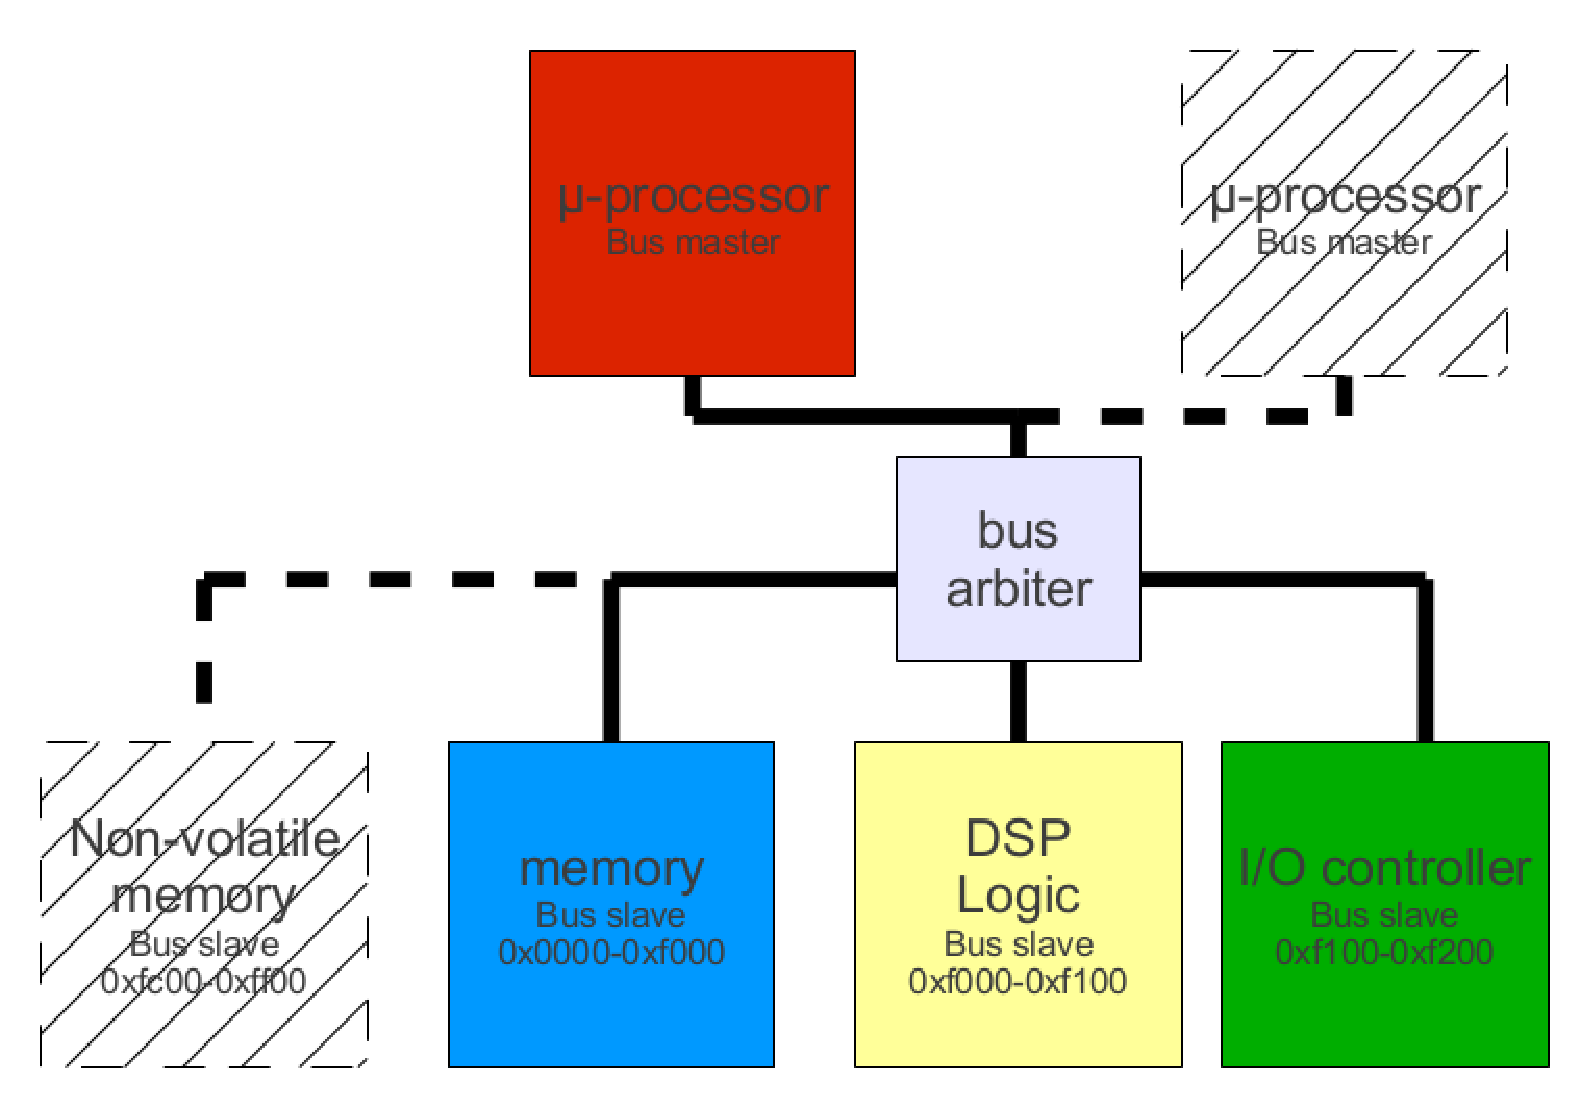
\includegraphics[scale=0.4]{soc_arch.eps}
\caption{Exemple d'implémentation de blocs IP dans un SoC}
\label{Fig_impl_blocs}
\end{center}
\end{figure}

Seule la description du circuit (les interconnexions entre les différents modules et les entrées/sorties du FPGA) est écrite à chaque fois que l'on change de carte et/ou de FPGA. Cette description peut être codée soit en VHDL ou en Verilog tout comme la description des blocs. Il s'agit souvent d'un \textit{memory-mapped} bus fournissant un accès aux registres de contrôle et aux mémoires. Dans notre cas, c'est un CSR bus conçu par Sébastien Bourdeauducq, à l'origine du projet \textit{Milkymist}.
\medskip

\begin{figure}
\begin{center}
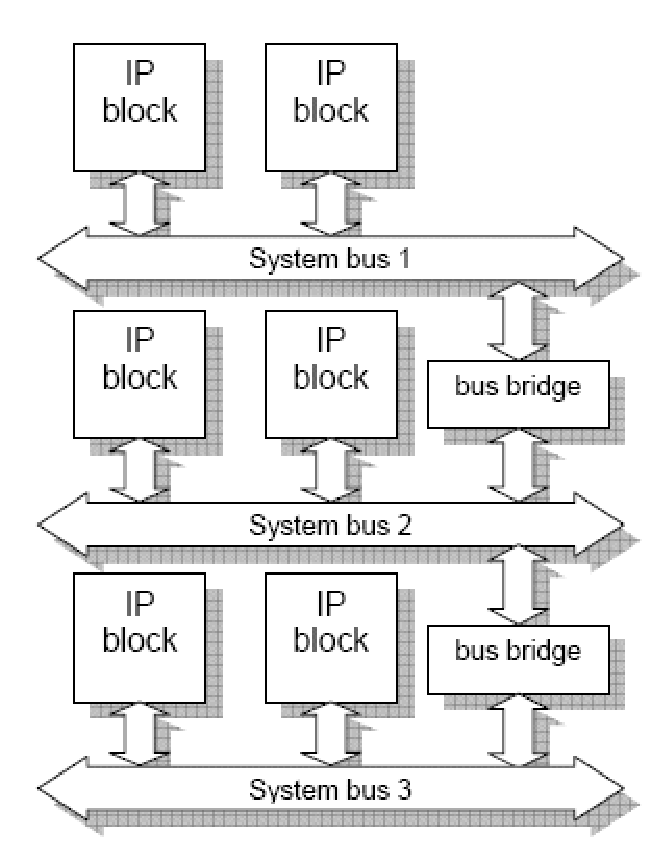
\includegraphics[scale=0.4]{soc_interconnect.eps}
\end{center}
\caption{Interconnexion des blocs IP par des bus}
\end{figure}

Dans notre cas, nous allons réutiliser plusieurs modules déjà implémentés. Tout d'abord, l'IP-Core LatticeMico32 (architecture RISC) déjà intégré dans \textit{Milkymist} et disponible gratuitement sous licence GNU GPL. Celui-ci nécessite tout de même quelques configurations de par sa généricité. On peut par exemple choisir selon ses besoins d'implémenter ou non, afin d'économiser des portes logiques, certaines parties dans l'unité de calcul (unité de multiplication, de décalage, activer les calculs signés, ...). On peut également changer la taille du bus, le nombre de registres, l'alimentation, le timing, la taille du cache, ...
Le GPIO, l'USART et d'autres éléments seront aussi réutilisés et configuré tout comme le processeur selon nos besoins.


Dans cette partie, nous avons vu l'énorme utilité de la généricité dans la description des IPs. Cet aspect est souvent utilisé dans l'industrie afin de créer un hardware spécifique au besoin d'un projet. On peut gagner par cette méthode énormément en efficacité face aux architectures non-spécialisées, ce qui permet à résultat égal de travailler avec une fréquence plus basse et du coup de moins consommer d'énergie.

